\chapter{Resultados}

Os resultados obtidos com as simulações estão descrito abaixo.

\section{Busca linear}

Na figura abaixo temos o resultado da simulação do algoritmo de busca linear em arranjos sequenciais de tamanhos diferentes, onde o tempo de execução médio foi medido. Fazendo um ajuste dos pontos da curva conseguimos determinar que o comportamento assintótico é linear.
\begin{figure}[H]
  \centering
  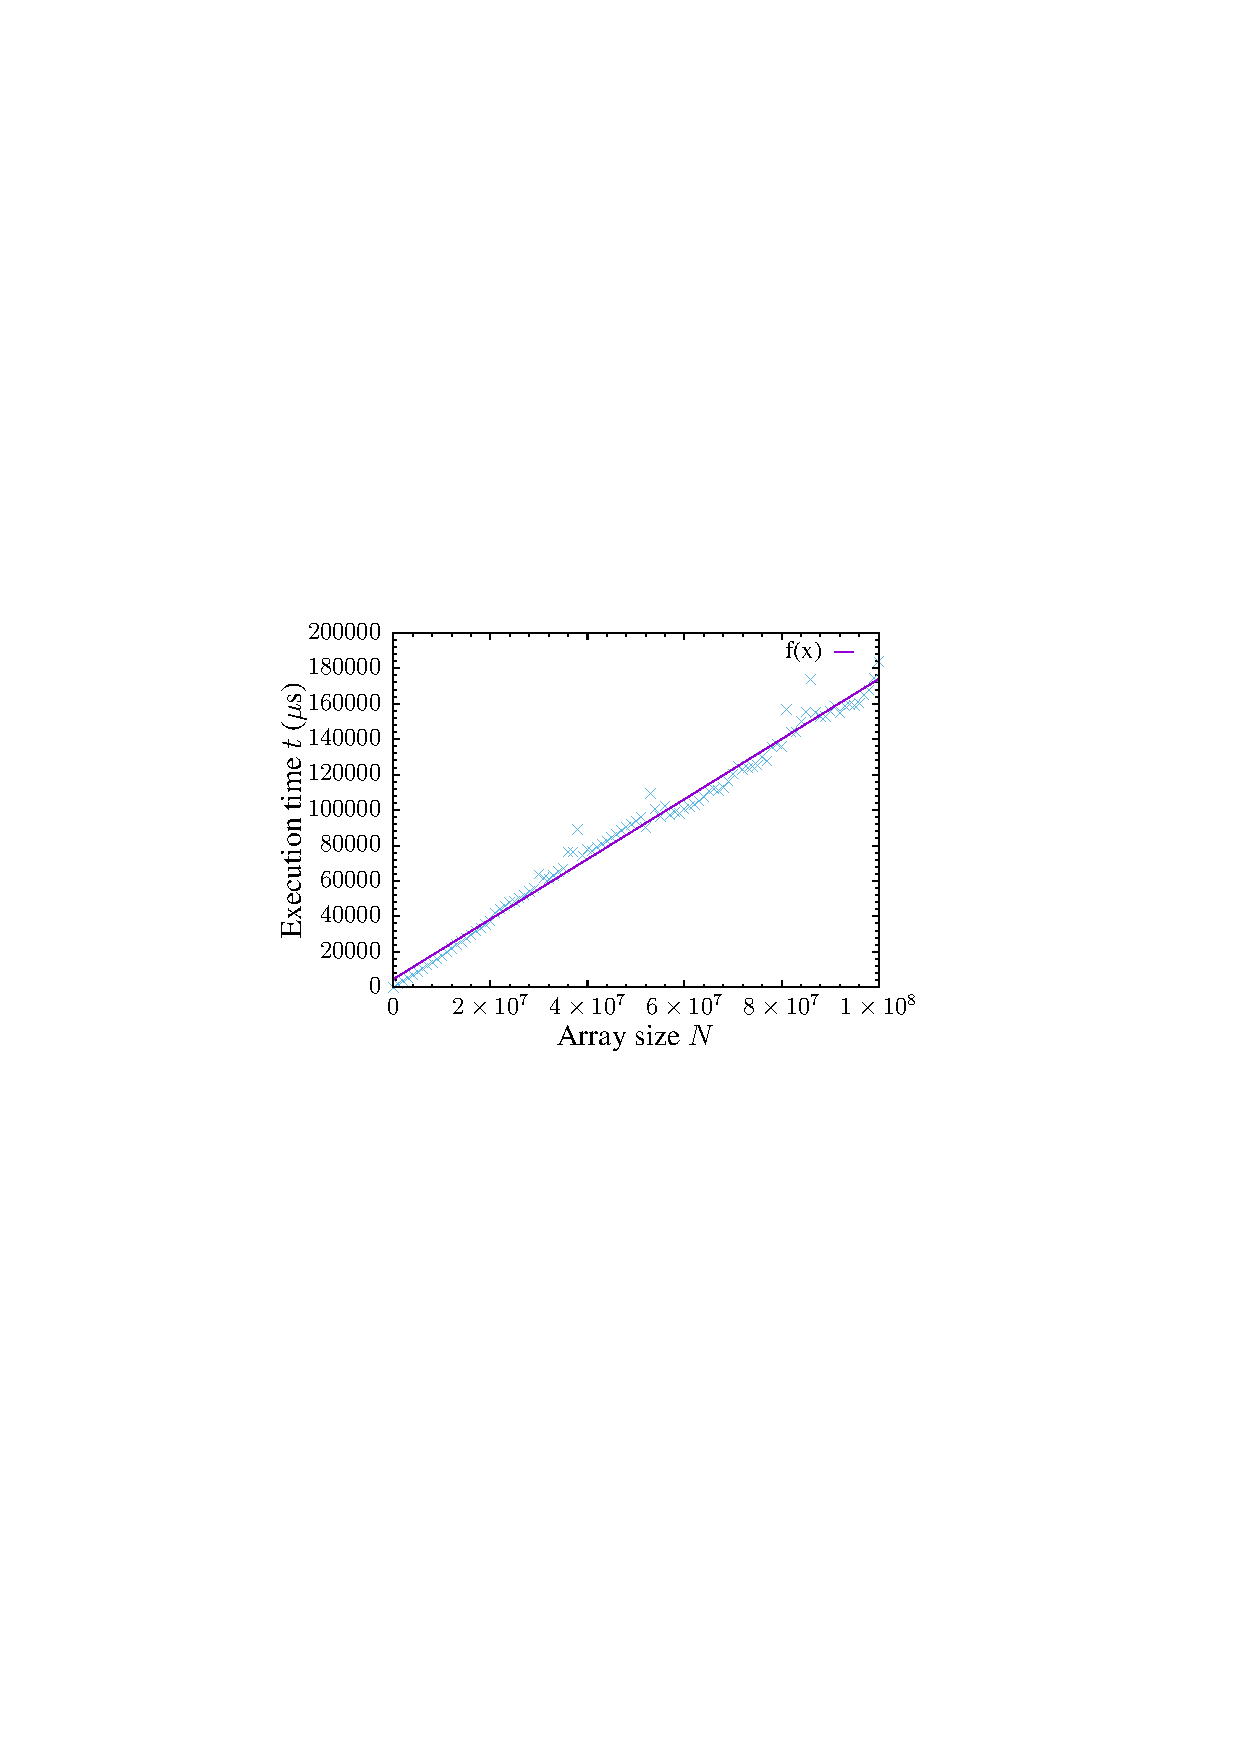
\includegraphics[scale=1.2]{../plots/lsearch_time.pdf}
 \caption{Comportamento assintótico da busca linear em relação ao tempo de execução médio (em milisegundos) a medida que o tamanho do arranjo sequencial $N$ aumenta.}
\end{figure} \label{fig:lseach_time}


\section{Busca binária}

Os resultado da simulação do algoritmo de busca binária em suas versões iterativa e recursiva em arranjos sequenciais de tamanhos diferentes seguem abaixo. Fazendo um ajuste dos pontos da curva de ambas as implementações conseguimos determinar que o comportamento é logarítmico.
\begin{figure}[H]
  \centering
  \includegraphics[scale=1.2]{../plots/bsearch_it_time.pdf}
  \caption{Comportamento assintótico da implementação iterativa da busca binária em relação ao tempo de execução médio (medido em nanosegundos).}
\end{figure} \label{fig:bseach_it_time}

\begin{figure}[H]
  \centering
  \includegraphics[scale=1.2]{../plots/bsearch_rec_time.pdf}
  \caption{Comportamento assintótico da implementação recursiva da busca binária em relação ao tempo de execução médio (medido em nanosegundos).}
\end{figure} \label{fig:bseach_rec_time}


\section{Busca ternária}

Nesta subseção, apresentamos os gráficos de tempo de execução em função do tamanho do arranjo para a busca ternária em suas versões iterativa e recursiva. Fazendo um ajuste dos pontos da curva de ambas as implementações conseguimos determinar que o comportamento é logarítmico.
\begin{figure}[H]
  \centering
  \includegraphics[scale=1.2]{../plots/tsearch_it_time.pdf}
%  \caption{Tempo vs...}
\end{figure} \label{fig:tseach_it_time}

\begin{figure}[H]
  \centering
  \includegraphics[scale=1.2]{../plots/tsearch_rec_time.pdf}
%  \caption{Tempo vs...}
\end{figure} \label{fig:tseach_rec_time}

\section{{\it Jump search}}

Na figura abaixo temos o resultado da simulação do algoritmo {\it jump search} em arranjos sequenciais de tamanhos diferentes, onde o tempo de execução médio foi medido. Fazendo um ajuste dos pontos da curva conseguimos determinar que o comportamento assintótico é linear.
\begin{figure}[H]
  \centering
  \includegraphics[scale=1.2]{../plots/jumpsearch_time.pdf}
%  \caption{Comportamento assintótico da {\it jump search} em relação ao tempo de execução médio (medido em milisegundos) a medida que o tamanho do arranjo sequencial $N$ aumenta.}
\end{figure} \label{fig:jumpsearch_time}

\section{Busca de Fibonacci}
